I dette afsnit SKRIV SENERE

\subsection{Grænseværdier af reele funktioner af delmængder af $\mathbb{R}$}%
\label{sub:Grænseværdi}
\begin{definition}[label=def:grænseværdi]{Grænseværdi for funktion}{}
  Antag $X \subseteq \mathbb{R}$, $f:X \to \mathbb{R}$, og $p$ er et fortætningspunkt af $X$.
  Et tal $L$ kaldes for grænseværdien af $f$ i $p$ og vi skriver
  \[
  \lim_{x \to p} f(x)= L,
  \] 
  hvis der for alle $\varepsilon >0$ eksisterer et tal $\delta >0$ sådan at når $x \in X$ og $0<\abs{x-p} < \delta  $, så gælder $\abs{f(x)-L} <\varepsilon $.  
\end{definition}

\begin{figure}[H]
\begin{center}
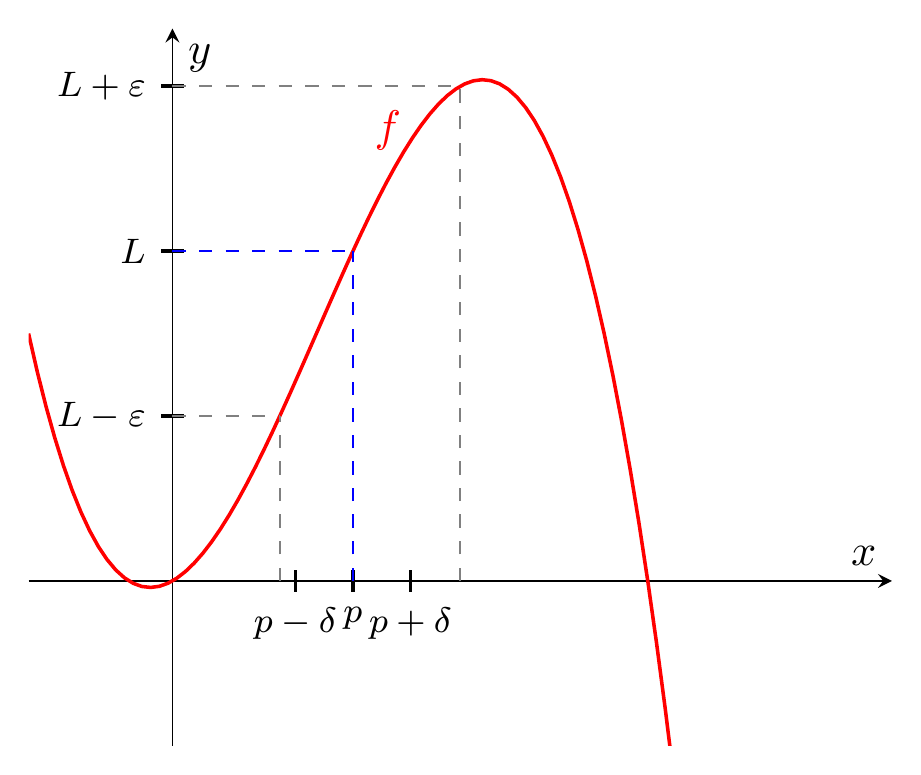
\begin{tikzpicture}[scale=1.6, transform shape]
\begin{axis}[xmin=-1, xmax=5, ymin=-2, ymax=6.7, axis lines=middle,
  xlabel=$x$,ylabel=$y$,
  xtick={0.8541,1.2541,1.6541},
  xticklabels={$p- \delta $, $p$, $p+\delta $},
  xticklabel style={anchor=north, font=\footnotesize},
  ytick={2,4,6},
  yticklabels={$L-\varepsilon $, $L$, $L+\varepsilon $},
  every major tick/.append style={thick, major tick length=5pt, black},
  yticklabel style={anchor=east, font=\footnotesize}
  ]
  \addplot[color=red, domain=-1:5, samples=100, thick]{-x^3 + 3*x^2+x} node[left, pos=0.15] {$f$};
  \draw[color=gray, dashed] (axis cs:0.7459,0) -- (axis cs:0.7459,2);
  \draw[color=gray, dashed] (axis cs:0,2) -- (axis cs:0.7459,2);
  \draw[color=gray, dashed] (axis cs:2,0) -- (axis cs:2,6);
  \draw[color=gray, dashed] (axis cs:0,6) -- (axis cs:2,6);
  \draw[color=blue, dashed] (axis cs:1.2541,0) -- (axis cs:1.2541,4);
  \draw[color=blue, dashed] (axis cs:0,4) -- (axis cs:1.2541,4);
\end{axis}
\end{tikzpicture}
\end{center}
\caption{$\varepsilon $-$\delta $-definition af funktionel grænseværdi}%
\label{fig:epsilondelta}
\end{figure}

Bemærk, at siden $p$ ikke behøver være i definitionsmængden $X$ (se eksempel \ref{exa:fortætningspunkter}), så kan grænseværdien for $f$ sagtens give mening i punkter, hvor selve $f$ ikke er defineret.

\begin{example}[label=exa:grænseværdi]{Grænseværdi i punkt, hvor funktion ikke er defineret}{}
 Lad funktionen $f:\{ x \in \mathbb{R}:x>0 \} \to \mathbb{R}$ være defineret ved
  \[
  f(x)= x^2.
  \] 
  Fra eksempel \ref{exa:fortætningspunkter} har vi, at $0$ er et fortætningspunkt af $\{ x \in \mathbb{R}:x>0 \} $. 
  Vores intuition fortæller os så, at
  \[
  \lim_{x \to 0} f(x)= 0.
  \] 
  Dette vil vi nu bevise stringent via definition \ref{def:grænseværdi}.

  For alle $\varepsilon >0$ vælger vi $\delta =\sqrt{\varepsilon } $. 
  Så har vi, at når $x \in \{ x \in \mathbb{R}:x>0 \} $ og $0<\abs{x-0} =\abs{x} <\delta $, så gælder
  \[
    \abs{f(x)-0} =\abs{x^2}=\abs{x}^2<\delta ^2=\varepsilon.
  \] 
  Altså har vi vist, at $\lim\limits_{x \to 0}f(x)=0$.
\end{example}

Det næste eksempel viser, at selv hvis et punkt $p$ tilhører definitionsmængden af en funktion $f$, så kan vi trods intuitionen godt have $\lim\limits_{x \to p} f(x) \neq f(p)$.

\begin{example}[label=exa:grænseværdi2]{Grænseværdi af funktion i punkt ulig funktionsværdien}{}
  
\end{example}

\subsection{Kontinuerte funktioner på intervaller}%
\label{sub:Kontinuert}


\begin{definition}{Begrænset funktion}{}
  
\end{definition}

